\chapter{Geheugenarchitectuur}
\label{architectuur}
De afzonderlijke geheugencellen zullen uiteindelijk samengebracht moeten worden in een geheel.
In dit hoofdstuk zal de algemene structuur besproken worden alsook de vrijheidsgraden die in hoofdstuk \ref{optimalisatie} onderzocht worden voor een optimaal werkend systeem. Ten slotte zullen ook nog de bouwblokken aangekaard worden die meer uitvoerig besproken worden in de volgende hoofdstukken. 

\section{Van transistorniveau tot systeemniveau}
Hoewel het hele systeem op de chip in weze bestaat uit transistoren en passieve componenten, zal dit nog onmogelijk te begrijpen vallen op zulke grote schaal.
Het is daarom aangewezen om meer abstractie te maken en de componenten vanop een hoger niveau te bekijken.

\subsection{Cel}
%Een tekst staat nooit alleen. Dit wil zeggen dat er zeker ook referenties
%nodig zijn. Dit kan zowel naar on-line documenten\cite{wiki} als naar
%boeken\cite{pratchett06:_good_omens}.
Zoals besproken in hoofdstuk \ref{cel} zal dit het bouwblok zijn dat het vaakst terug zal te vinden zijn op het geheugensysteem.
De cel bestaat uit een memristor en een transistor. De geheugencel heeft drie terminals: de gate van de transistor, die zal verbonden worden met een wordline, de source van de transistor, die zal verbonden worden met een sourceline en tenslotte de terminal van de memristor, die zal verbonden worden met een bitline.
Een cel wiens memristor zich in een willekeurige resistieve staat bevindt is een datacel, terwijl de memristor van referentiecellen in een voorgeprogrammeerde en dus gekende resistieve staat verkeert.

\subsection{Branch}
In een branch worden er een bepaald aantal datacellen verbonden aan één BL en één SL. Dit aantal wordt \emph{Number of WL per Branch} (NoWLpB) genoemd en is een van de vrijheidsgraden van de geheugenarchitectuur. Naast alle datacellen is er ook nog één referentiecel verbonden aan de BL en SL van de branch.
Elke BL wordt via een pMOS-transistor verbonden aan de voedingspanning Vdd (al dan niet met een impedantie ertussen) en via een nMOS-transistor aan de grondspanning Vss. In dit werk is er enkel een nMOS-transistor die de SL verbindt met Vss.\footnote{In een volledig geheugensysteem zou de SL via een pMOS ook nog verbonden zijn met een niet onderzochte spanningsknoop Vdd\_write. De pMOS zou dan worden aangezet voor schrijfwerking.}
Ter illustratie wordt de samenhang tussen cel en branch getoond in figuur \ref{fig:cellbranch}.

\begin{figure}
  \centering
  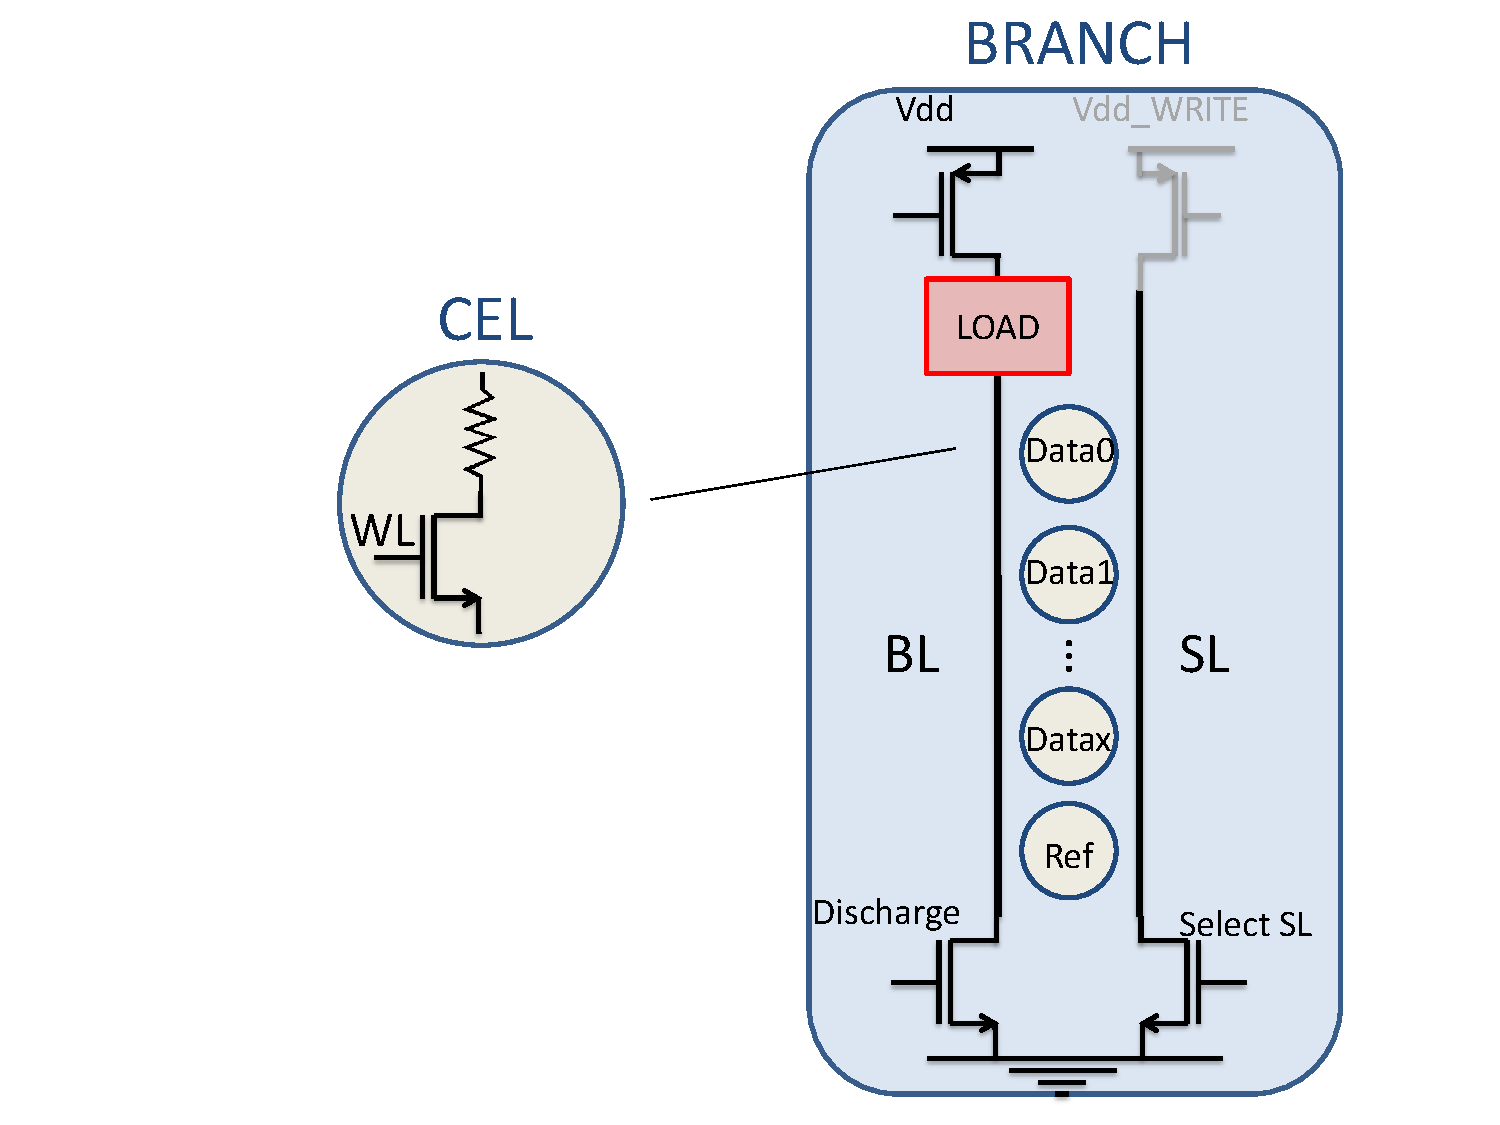
\includegraphics[scale=0.3]{../fig/hfdstk-architecture-cell-branch.pdf}
  \caption{Een geheugencel en een branch}
  \label{fig:cellbranch}
\end{figure}

\subsection{Local Block}
Verschillende BLs en SLs worden samengebracht in een Local Block, waarvan de vrijheidsgraad \emph{Number of Bit Lines per Local Block} (NoBLpLB) heet. In een LB bevinden er zich dus NoBLpLB x NoWLpB datacellen en NoBLpLB referentiecellen. Ook zitten er in een Local Block zowel BL- als WL-decoders.
De structuur van een Local Block is geïllustreerd op figuur \ref{fig:LB}.
De uitgangen van de WL-decoders worden gebufferd (meer hierover in hoofdstuk \ref{periphery}) en vervolgens aangesloten op de WLs zelf: naarmate NoBLpLB groter wordt, gaat de WL-capaciteit immers lineair toenemen.
Zoals blijkt uit hoofdstuk \ref{loadanalysis}, behoeven de uitgangen van de BL-decoder geen buffering en kunnen deze worden aangesloten zoals getoond op figuur \ref{fig:BL-decoder-data} en \ref{fig:BL-decoder-ref}.
Aangezien een LB zowel data- als referentiecellen bevat, gaat een LB twee werkingsmodes hebben: een mode waarbij er één datacel wordt aangesproken en een mode waarbij er een bepaald aantal referentiecellen in parallel wordt aangesproken.
Het controlesignaal LB\_enable\_x bepaalt volgens welke modus het LB zich gaat gedragen.

\begin{figure}
  \centering
  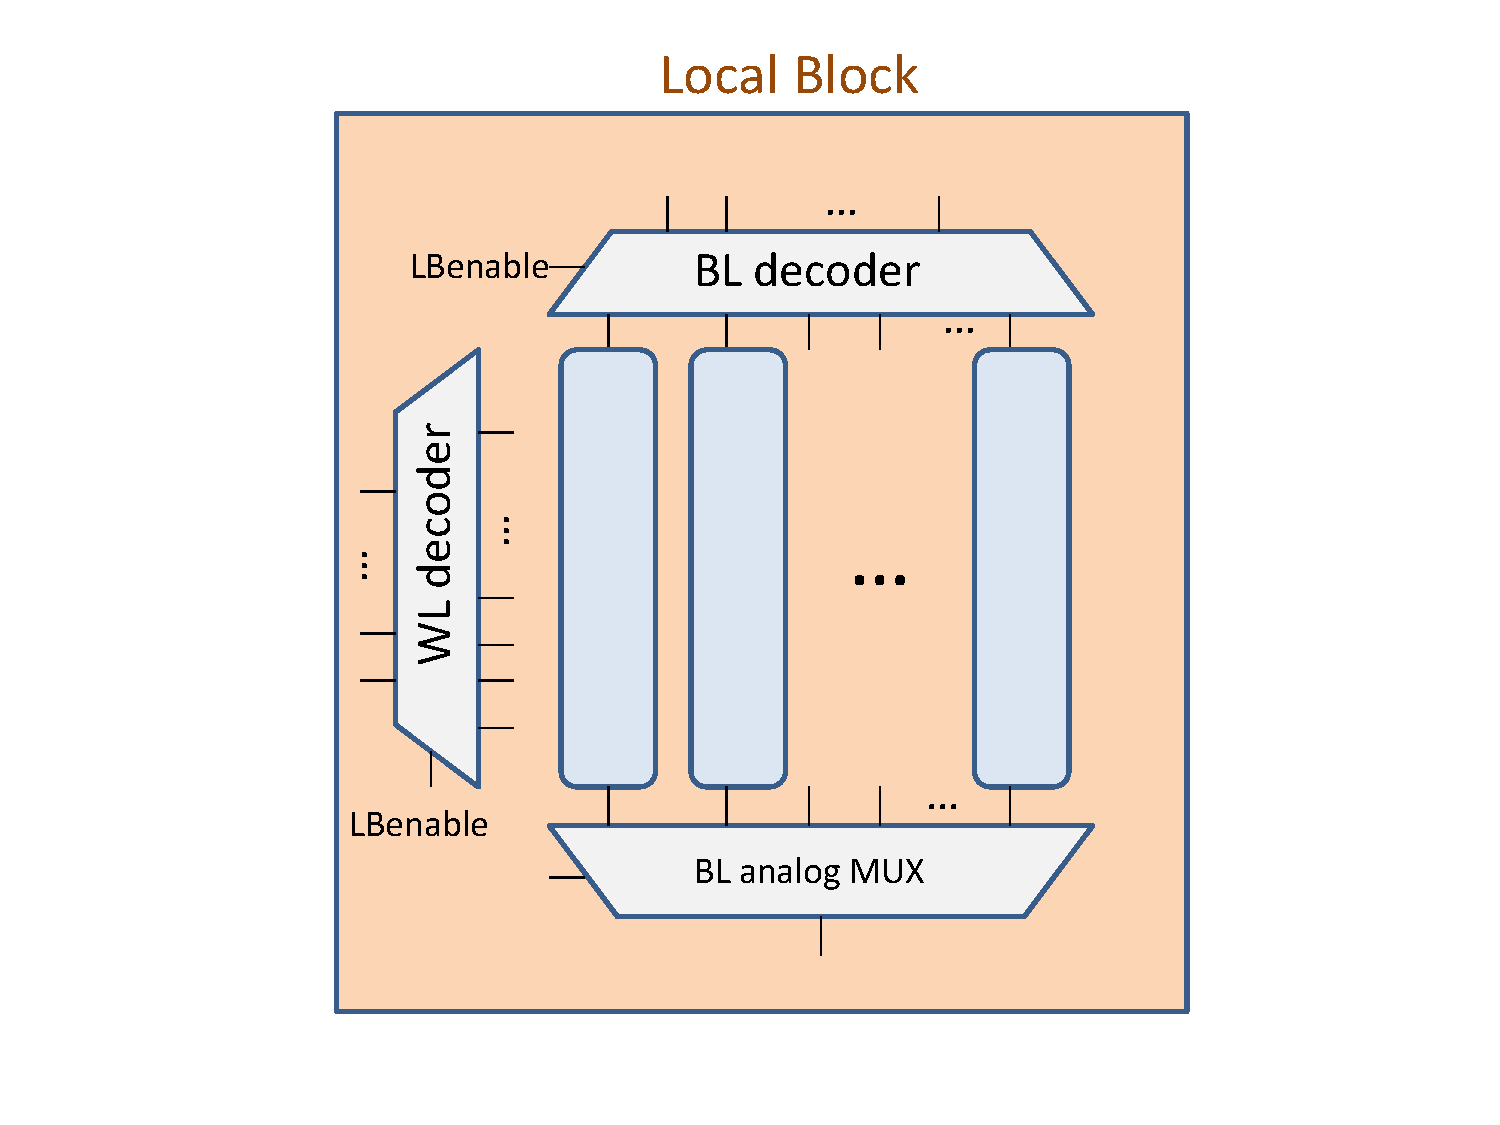
\includegraphics[scale=0.3]{../fig/hfdstk-architecture-localblock.pdf}
  \caption{Een Local Block}
  \label{fig:LB}
\end{figure}

\subsection{Global Block}
Een Global Block bestaat uit twee LBs en een sense amplifier (SA). In het ene LB gaat er een datasignaal geproduceerd worden, in het andere een referentiesignaal (zie figuur \ref{fig:GB}. Vervolgens gaat de SA dit kleine signaalverschil versterken tot een zuivere rail-to-rail output.
Aan de uitgang van het GB verschijnen dan ook de opgevraagde bits.
%\section{Figuren}
%Figuren worden gebruikt om illustraties toe te voegen. Dit is dan ook de
%manier om beeldmateriaal toe te voegen zoals getoond wordt in
%figuur~\ref{fig:logo}.
%
%\begin{figure}
%  \centering
%  
\includegraphics{logokul}
%  \caption{Het KU~Leuven logo.}
%  \label{fig:logo}
%\end{figure}
%
%\section{Tabellen}
%Tabellen kunnen gebruikt worden om informatie op een overzichtelijke te
%groeperen. Een tabel is echter geen rekenblad! Vergelijk maar eens
%tabel~\ref{tab:verkeerd} en tabel~\ref{tab:juist}. Welke tabel vind jij het
%duidelijkst?
%
%\begin{table}
%  \centering
%  \begin{tabular}{||l|lr||} \hline
%    gnats     & gram      & \$13.65 \\ \cline{2-3}
%              & each      & .01 \\ \hline
%    gnu       & stuffed   & 92.50 \\ \cline{1-1} \cline{3-3}
%    emu       &           & 33.33 \\ \hline
%    armadillo & frozen    & 8.99 \\ \hline
%  \end{tabular}
%  \caption{Een tabel zoals het niet moet.}
%  \label{tab:verkeerd}
%\end{table}
%
%\begin{table}
%  \centering
%  \begin{tabular}{@{}llr@{}} \toprule
%    \multicolumn{2}{c}{Item} \\ \cmidrule(r){1-2}
%    Animal    & Description & Price (\$)\\ \midrule
%    Gnat      & per gram    & 13.65 \\
%              & each        & 0.01 \\
%    Gnu       & stuffed     & 92.50 \\
%    Emu       & stuffed     & 33.33 \\
%    Armadillo & frozen      & 8.99 \\ \bottomrule
%  \end{tabular}
%  \caption{Een tabel zoals het beter is.}
%  \label{tab:juist}
%\end{table}


\section{Besluit van dit hoofdstuk}
Als je in dit hoofdstuk tot belangrijke resultaten of besluiten gekomen
bent, dan is het ook logisch om het hoofdstuk af te ronden met een
overzicht ervan. Voor hoofdstukken zoals de inleiding en het
literatuuroverzicht is dit niet strikt nodig.

%%% Local Variables: 
%%% mode: latex
%%% TeX-master: "masterproef"
%%% End: 
